\chapter{使用指南}

\section{脚注}
使用\textbackslash footnote来插入一个脚注\footnote{我是一条测试用的脚注}\footnote{真巧,我也是}\footnote{还有我}

\section{层级}
由于排版需要(懒得折腾)本模板只支持到subsection级别,标号规则遵从格式要求,如需要使用更深层标题,请改用列表环境并注意
指定所需格式。

\section{列表环境}

enumerate环境可以生成有序列表,默认序号格式如下:

\begin{enumerate}
\item 默认
\item 输出
\item 的
\item 列表
\end{enumerate}

通过控制label选项,可以输出不同格式的序号:

\begin{lstlisting}{language=TeX}
  \begin{enumerate}[label=(\arabic*)] % (1) (2) ...
\end{lstlisting}


下面是由此生成的列表

\begin{enumerate}[label=(\arabic*)]
\item 不同样子
\item 的
\item 列表
\end{enumerate}

无序号列表由itemize环境生成

\begin{itemize}
\item firstItem
\item seconItem
\item and so on
\end{itemize}

\section{代码环境示例}

下面是用listings包生成的一段C语言代码
\begin{lstlisting}{language=C}
if (i<=0) then i := 1;
if (i>=0) then i := 0;
if (i<>0) then i := 0;
\end{lstlisting}

\section{表格环境}

按规范,表格应为三线式,请依照格式制作表格\footnote{注释每页独立编号}

\begin{table}[htbp]
  \centering
  \caption{标题}
    \begin{tabular}{rrrrrr}
    \toprule
    test  & test  & test  & test  & test  & test \\
    \midrule
    test  & test  & test  & test  & test  & test \\
    test  & test  & test  & test  & test  & test \\
    test  & test  & test  & test  & test  & test \\
    test  & test  & test  & test  & test  & test \\
    test  & test  & test  & test  & test  & test \\
    test  & test  & test  & test  & test  & test \\
    \bottomrule
    \end{tabular}%
  \label{tab:addlabel}%
\end{table}%

\section{输入数学公式}
\begin{equation}
E=mc^2
\end{equation}

引用公式需要在标号外加括号,为了保证引用格式的正确,请使用amsmath包提供的 \textbackslash eqref来生成公式
引用而非\textbackslash ref

需要对齐的公式环境 \eqref{eq_test1} 到 \eqref{eq_test3}
\begin{align}
a &= 1 \label{eq_test1}\\
b &= 2 \label{eq_test2}\\
c &= 299792458\,\text{m/s} \label{eq_test3}
\end{align}

\section{带圈数字}
\textbackslash circnum通过映射数字实现了比较漂亮的带圈数字输出,主要用于注释及enumerate环境。
对于大于10的数字支持可能存在问题,请谨慎使用。

\begin{itemize}
  \item 1-10的数字将将其映射为对应字符\circnum{1}\circnum{2}\circnum{3}\circnum{4}\circnum{5}\circnum{6}\circnum{7}\circnum{8}\circnum{9}\circnum{10}
  \item 其余数字利用\textbackslash textcircled加框,同时对数字位置作了微调\circnum{0}\circnum{20}\circnum{99}
\end{itemize}

\section{插图示例}

\begin{figure}[htbp]
  \centering
  \subfigure[高德纳]{ 
    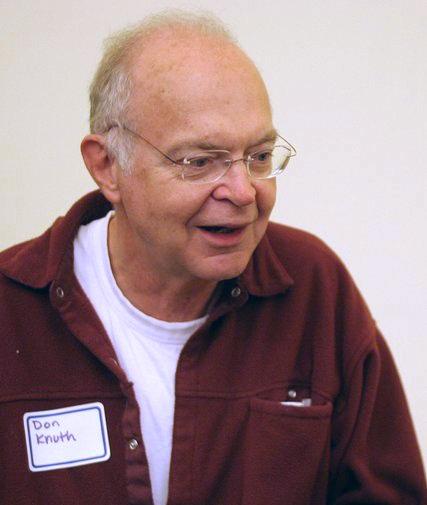
\includegraphics[height=6cm]{figure/Knuth.jpg}
  }
  \subfigure[莱斯利·兰波特]{ 
    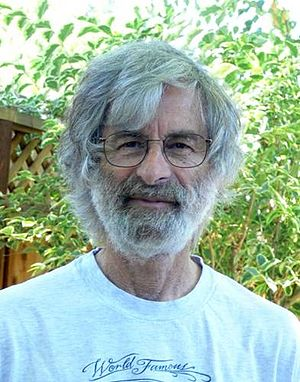
\includegraphics[height=6cm]{figure/Leslie_Lamport.jpg}
  }
  \caption{高德纳和莱斯利·兰波特,\TeX{}和\LaTeX{}的开发者}
\end{figure}

\section{参考文献}
参考文献格式部分参考了\href{https://github.com/ustctug/gbt-7714-2015}{GB/T 7714-2015 BibTeX Style},并进行了一部分改动,
整理比较仓促,如使用中发现了问题,请尽快与作者联系。

\section{长表格}

跨页长表格用longtable环境产生,请参考表 \ref{tab-data}进行长表格制作。

\begin{center}
\begin{longtable}{lrr}
\caption{我是一个长表格}\label{tab-data}\\
\toprule
Sample  & Sample & Sample \\
\midrule
\endfirsthead
\multicolumn{3}{c}{\hfill (接上页) \hfill 续表 \ref{tab-data}}\\
\toprule
Sample  & Sample & Sample \\
\midrule
\endhead
\bottomrule
\multicolumn{3}{c}{(接下页)}
\endfoot
\bottomrule
\endlastfoot
1234567 & 2     & 3.00000000000000E+00 \\
1234567 & 4     & 9.00000000000000E+00 \\
1234567 & 8     & 2.70000000000000E+01 \\
1234567 & 16    & 8.10000000000000E+01 \\
1234567 & 32    & 2.43000000000000E+02 \\
1234567 & 64    & 7.29000000000000E+02 \\
1234567 & 128   & 2.18700000000000E+03 \\
1234567 & 256   & 6.56100000000000E+03 \\
1234567 & 512   & 1.96830000000001E+04 \\
1234567 & 1024  & 5.90490000000003E+04 \\
1234567 & 2048  & 1.77147000000001E+05 \\
1234567 & 4096  & 5.31441000000003E+05 \\
1234567 & 8192  & 1.59432300000001E+06 \\
1234567 & 16384 & 4.78296900000003E+06 \\
1234567 & 32768 & 1.43489070000001E+07 \\
1234567 & 65536 & 4.30467210000003E+07 \\
1234567 & 131072 & 1.29140163000001E+08 \\
1234567 & 262144 & 3.87420489000003E+08 \\
1234567 & 524288 & 1.16226146700001E+09 \\
1234567 & 1048576 & 3.48678440100003E+09 \\
1234567 & 2097152 & 1.04603532030001E+10 \\
1234567 & 4194304 & 3.13810596090003E+10 \\
1234567 & 8388608 & 9.41431788270006E+10 \\
1234567 & 16777216 & 2.82429536481002E+11 \\
1234567 & 33554432 & 8.47288609443006E+11 \\
1234567 & 67108864 & 2.54186582832902E+12 \\
1234567 & 134217728 & 7.62559748498706E+12 \\
1234567 & 268435456 & 2.28767924549612E+13 \\
1234567 & 72434964.49 & 6.86303773648836E+13 \\
1234567 & 76108137.14 & 2.05891132094651E+14 \\
1234567 & 79781309.79 & 6.17673396283953E+14 \\
1234567 & 83454482.44 & 1.85302018885186E+15 \\
1234567 & 87127655.09 & 5.55906056655558E+15 \\
1234567 & 90800827.74 & 1.66771816996667E+16 \\
1234567 & 94474000.39 & 5.00315450990001E+16 \\
1234567 & 98147173.04 & 1.50094635297001E+17 \\
1234567 & 101820345.7 & 4.50283905891003E+17 \\
1234567 & 105493518.3 & 1.35085171767301E+18 \\
1234567 & 109166691 & 4.05255515301903E+18 \\
1234567 & 112839863.6 & 1.21576654590571E+19 \\
1234567 & 116513036.3 & 3.64729963771713E+19 \\
1234567 & 120186208.9 & 1.09418989131514E+20 \\
1234567 & 123859381.6 & 3.28256967394542E+20 \\
1234567 & 127532554.2 & 9.84770902183626E+20 \\
1234567 & 131205726.9 & 2.95431270655087E+21 \\
1234567 & 134878899.5 & 8.86293811965264E+21 \\
1234567 & 138552072.2 & 2.65888143589579E+22 \\
1234567 & 142225244.8 & 7.97664430768737E+22 \\
1234567 & 145898417.5 & 2.39299329230621E+23 \\
1234567 & 149571590.1 & 7.17897987691863E+23 \\
1234567 & 153244762.8 & 2.15369396307559E+24 \\
1234567 & 156917935.4 & 6.46108188922677E+24 \\
1234567 & 160591108.1 & 1.93832456676803E+25 \\
1234567 & 164264280.7 & 5.81497370030409E+25 \\
1234567 & 167937453.4 & 1.74449211009123E+26 \\
1234567 & 171610626 & 5.23347633027369E+26 \\
1234567 & 175283798.7 & 1.57004289908211E+27 \\
\end{longtable}
\end{center}

